\section{复杂的论证性语段}

\begin{logicbox}[title=引言]
\textit{复杂的论证性语段是我们在实践中常见的推理形式,它们涉及多个前提和结论的交织,通过掌握分析方法,我们能更清晰地理解和评估这些论证。}
\end{logicbox}

在现实世界中,论证往往具有相当的复杂性,远超简单的前提-结论模式。这些复杂论证具有以下特征:

\begin{theorembox}[title=复杂论证的结构特征]
\logicemph{多层次结构}:
\begin{itemize}
  \item 由多个子论证组合而成
  \item 形成\logicterm{论证链}或\logicterm{论证网络}
  \item 存在多条推理路径通向最终结论
\end{itemize}

\logicemph{命题的多重角色}:
\begin{itemize}
  \item 某些命题仅作为\logicterm{前提}
  \item 某些命题仅作为\logicterm{结论}
  \item 某些命题既作为前提又作为\logicterm{分结论}(中间结论)
\end{itemize}
\end{theorembox}

\begin{theorembox}[title=图示法的作用与限制]
\logicemph{图示法的优势}:
\begin{itemize}
  \item 直观展现论证的逻辑结构
  \item 清晰显示前提与结论的关系
  \item 便于识别推理的薄弱环节
\end{itemize}

\logicwarn{方法的限制}:
\begin{itemize}
  \item \logicwarn{不存在机械化的图示构建方法}
  \item 同一语段可能有多种合理的解释
  \item 需要分析者的判断和理解能力
\end{itemize}
\end{theorembox}

\subsection{复杂语段分析方法}

分析复杂论证需要系统的方法和清晰的思路。我们的\logicemph{分析策略}包括:

\begin{theorembox}[title=复杂论证分析步骤]
\begin{enumerate}
  \item \logicterm{理解推理流程}:把握作者的整体论证思路
  \item \logicterm{识别命题角色}:确定每个命题在论证中的功能
  \item \logicterm{标记命题编号}:为便于分析,给关键命题编号
  \item \logicterm{构建逻辑图示}:用图形展现前提与结论的关系
  \item \logicterm{评估推理有效性}:判断结论是否真正从前提推出
\end{enumerate}
\end{theorembox}

下面我们通过一个具体例子来演示这种分析方法。这个论证具有典型的复杂结构:\logicemph{最终结论出现在语段开头},有四个前提直接支持这个结论,其中两个前提本身又是分结论,分别得到其他前提的支持:

\begin{displayquote}
(1)看来, 用动物实验进行科学研究的做法并不是不必要的或靠不住的; (2)在使用脊椎动物进行实验之前, 实验的草案必须经过包括一名兽医和一名公众代表在内的公共机构委员会进行的再审查, 并且(3)在研究期间, 动物的医疗和卫生情况得到定期监测。(4)研究者需要健康的动物进行科学研究和医学研究, 因为(5)不健康的动物可能导致错误的研究结果。这激励(6)科学家确保他们使用的任何动物健康并且营养良好。此外, (7)用动物进行研究是昂贵的, 因为(8)料学研究的资金受到限制, (9)只有高质量的研究才能通过有力的竞争获得对研究的支持。$^{[49]}$
\end{displayquote}

\begin{examplebox}[title=动物实验论证的结构分析]
\logicemph{论证结构解析}:
\begin{itemize}
  \item \logicterm{最终结论}:(1) 动物实验是必要且可靠的
  \item \logicterm{直接支持前提}:(2) 审查制度、(3) 监测制度、(6) 科学家的激励、(7) 研究成本高
  \item \logicterm{分结论及其支持}:
    \begin{itemize}
      \item (6) 由 (4) 和 (5) 支持
      \item (7) 由 (8) 和 (9) 支持
    \end{itemize}
\end{itemize}
\end{examplebox}

下面的图示展示了这段话的逻辑结构。\logicemph{图示解读方法}:从图中最高处(逻辑起点)开始,沿着箭头方向追踪推理路径,可以看到多条推理线路如何汇聚到最终结论。

\begin{center}
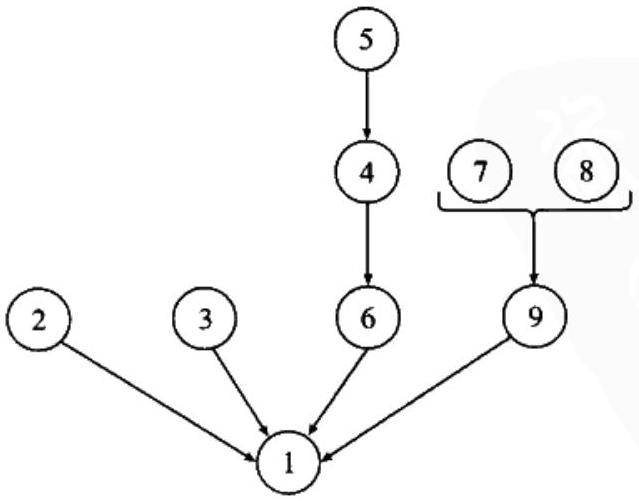
\includegraphics[width=\textwidth]{images/2025_05_15_6a28331d5e7c993ad07ag-072.jpg}
\end{center}

\subsection{处理重复和强调的命题}

在复杂论证中,我们经常遇到\logicterm{命题重复}和\logicterm{强调}现象,这给分析带来了额外的挑战。

\begin{theorembox}[title=处理重复命题的策略]
\logicemph{重复出现的原因}:
\begin{itemize}
  \item \logicterm{强调重要观点}:作者希望突出关键命题
  \item \logicterm{修辞效果}:增强说服力和表达力
  \item \logicterm{逻辑需要}:同一命题在不同推理环节中发挥作用
\end{itemize}

\logicemph{分析方法}:
\begin{itemize}
  \item 用\logicwarn{相同编号}标记相同命题的不同表述
  \item 识别命题的\logicterm{核心含义},忽略表达方式的差异
  \item 在图示中\logicemph{合并}重复出现的命题
\end{itemize}
\end{theorembox}

下面的例子展示了一个包含大量重复的复杂论证,它由三个清晰的子论证构成:

\begin{displayquote}
(1)宇宙大爆炸理论正在瓦解……(2)根据正统知识, 宇宙起源于大爆炸——200 亿年前的一次巨大的、非常匀称的爆炸。问题是(3)天文学家通过进一步观测证实: 现存的巨大星系团因为体积太大, 完全不可能在仅仅 200 亿年时间中形成……通过人造卫星所收集的新材料的研究, 以及较早前的地面测量表明(4)星系聚集成绵延数十亿光年的巨大带状, 并且(5)星系之间有亿方光年的距离。因为(6)据观测, 星系移动的速度远不及光速, 数学家证明(7)聚集成这么大的物质团必须要经过至少 1000 亿年时间——是假设的大爆炸时间的五倍……(3)像那么大的一种结构现在看来不可能在 200亿年时间中形成……(2)大爆炸理论认为, 物质均匀地散布在宇宙中。而与这种理想理论相反, (3)这么巨大的星丛无法这么快地形成。$^{[50]}$
\end{displayquote}

\begin{examplebox}[title=大爆炸理论论证的结构分析]
\logicemph{重复命题的识别}:
\begin{itemize}
  \item 命题(2):大爆炸理论的基本观点(出现3次)
  \item 命题(3):巨大结构无法快速形成(出现3次)
  \item 其他命题各出现1-2次
\end{itemize}

\logicemph{推理链条分析}:
\begin{enumerate}
  \item \logicterm{观察证据}:(4)(5)(6) → (7) 形成时间计算
  \item \logicterm{科学推论}:(7) → (3) 结构形成困难
  \item \logicterm{理论评判}:(2)(3) → (1) 理论瓦解
\end{enumerate}
\end{examplebox}

下面的图示展示了这段话的逻辑关系:

\begin{center}
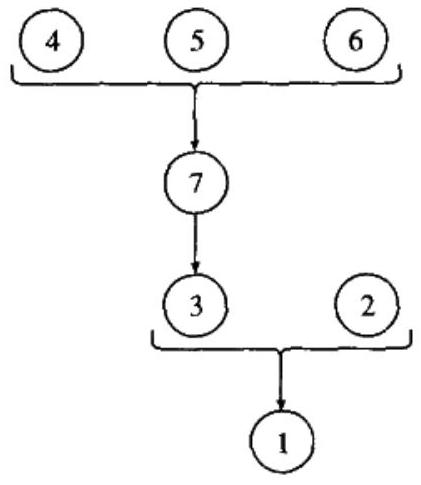
\includegraphics[width=\textwidth]{images/2025_05_15_6a28331d5e7c993ad07ag-073.jpg}
\end{center}

\subsection{处理浓缩的前提}

在复杂论证分析中,我们还需要处理\logicterm{浓缩前提}的问题。

\begin{theorembox}[title=浓缩前提的特征与处理]
\logicemph{浓缩形式的表现}:
\begin{itemize}
  \item 用\logicterm{名词短语}代替完整命题
  \item 省略主语、谓语或其他成分
  \item 依赖语境理解完整含义
\end{itemize}

\logicemph{处理策略}:
\begin{itemize}
  \item \logicterm{重构完整命题}:将短语扩展为完整的陈述句
  \item \logicterm{明确逻辑关系}:确定浓缩前提在推理中的作用
  \item \logicterm{保持原意}:扩展时不改变原始含义
\end{itemize}
\end{theorembox}

下面的例子展示了浓缩前提与重复命题同时出现的复杂情况。例如,短语"在大气中的散射"作为前提(4),需要重构为"太阳的能量在大气中散射":

\begin{displayquote}
(1)太阳能汽车只是一种试验性的装置, 其他什么都不是。(2)太阳的能量太弱以至于不能发动甚至是日常使用的迷你汽车。(3)进入大气层的太阳能量大约为每平方码 1 千瓦。因为(4)在大气中的散射, 又因为(5)地球上的任何地方一天中平均只有半天时间受到阳光的照射, (6)每天接收的太阳功率平均为 $1 / 6$ 千瓦时到 4千瓦时 $\cdots \cdots$ 对通常规格的汽车的检测表明, (7)若使一辆电车勉强能够工作, 其电池组需要 300 千瓦时的能量。因此, (8)充满汽车电池必须有 40 平方码的原电池, 大约是一辆拖拉机的拖车顶部的尺寸。(1)除了用于昂贵的试验汽车外, 太阳能没有指望成为任何汽车的动力, 太阳能汽车不是一项待开发的技术。这就是结论。$^{[51]}$
\end{displayquote}

\begin{examplebox}[title=太阳能汽车论证的结构分析]
\logicemph{论证特点}:
\begin{itemize}
  \item \logicterm{结论重复}:命题(1)在开头和结尾都出现,但表述略有不同
  \item \logicterm{浓缩前提}:命题(4)"在大气中的散射"需要扩展理解
  \item \logicterm{数据支撑}:大量具体数据支持能量计算
\end{itemize}

\logicemph{推理结构}:
\begin{itemize}
  \item 从太阳能量密度(3)出发
  \item 考虑损失因素(4)(5)得出实际功率(6)
  \item 结合汽车需求(7)计算所需面积(8)
  \item 最终得出实用性结论(1)
\end{itemize}
\end{examplebox}

这段话的图示为:

\begin{center}
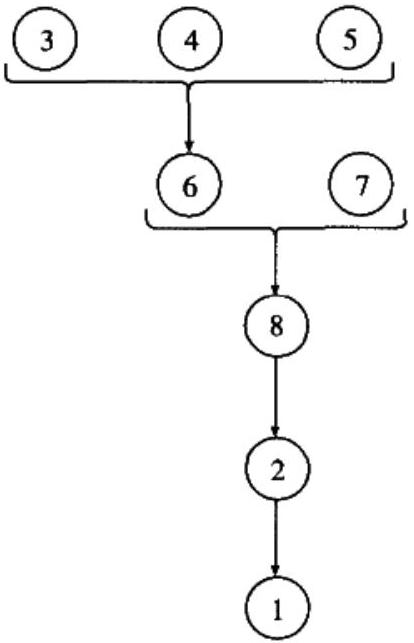
\includegraphics[width=\textwidth]{images/2025_05_15_6a28331d5e7c993ad07ag-074.jpg}
\end{center}

\subsection{融贯的复杂论证分析}

在分析复杂论证时,我们会发现一些语段尽管包含众多前提和分结论,但展现出\logicemph{高度的逻辑融贯性}。这种融贯性体现在:
\begin{itemize}
  \item 每个命题都有明确的逻辑作用
  \item 推理路径清晰且相互支撑
  \item 整体结构服务于统一的论证目标
\end{itemize}

下面是一个典型的融贯复杂论证,来自一位女编辑为其争议性编辑方针所做的辩护:

\begin{displayquote}
本刊(《新英格兰医学杂志》)的主张是(1)不发表不道德的研究报告,忽略它们的料学价值……

我们的主张有三个理由。首先,(2)如果普遍坚持这个主张,只发表合乎道德的研究文章,将会阻止不合乎道德的研究工作的开展。(3)文章的发表是医学研究奖赏制度的一个重要部分。(4)如果研究者知道他们不合乎道德的研究成果不能发表,他们就不会去做不道德的研究。(5)而相反的做法将有助于导致更多的不道德研究工作的开展,因为,如我已表明的,(6)这样的研究可能比较容易开展,因而(7)可能使从事不道德研究工作的人处于有利的竞争地位。其次,(8)即使发表不道德的研究成果不妨碍发表合乎道德的研究成果,为了坚持把合乎道德放在研究第一位的原则,也应该拒绝不道德的研究。(9)如果允许有所松动,我们将逐渐变得习惯于发表不道德的研究成果,并且(10)这将导致对发表合乎道德的研究成果的极大妨碍。最后,(11)对不道德研究成果的拒绝,有利于使社会普遍注意到,甚至某些科学家也不懂得科学研究应是文明的基本尺度。(12)知识尽管很重要,但对一个公平公正的社会来说知识或许远不及得到知识的方法重要。$^{[52]}$
\end{displayquote}

\begin{examplebox}[title=医学期刊编辑方针论证分析]
\logicemph{论证结构特点}:
\begin{itemize}
  \item \logicterm{三重支撑}:(2)(8)(11)三个主要命题直接支持结论(1)
  \item \logicterm{层次清晰}:每个主要前提都有相应的支持前提
  \item \logicterm{逻辑完整}:从预防效果、原则坚持、社会影响三个角度全面论证
\end{itemize}

\logicemph{论证策略}:
\begin{enumerate}
  \item \logicterm{预防论证}:发表政策影响研究行为
  \item \logicterm{原则论证}:道德标准的重要性
  \item \logicterm{社会论证}:科学研究的文明责任
\end{enumerate}
\end{examplebox}

这个复杂但推理缜密的语段展现了高质量论证的特征:每个命题都有明确的逻辑作用,共同服务于统一的论证目标。下面的图示展示了其逻辑结构:

\begin{center}
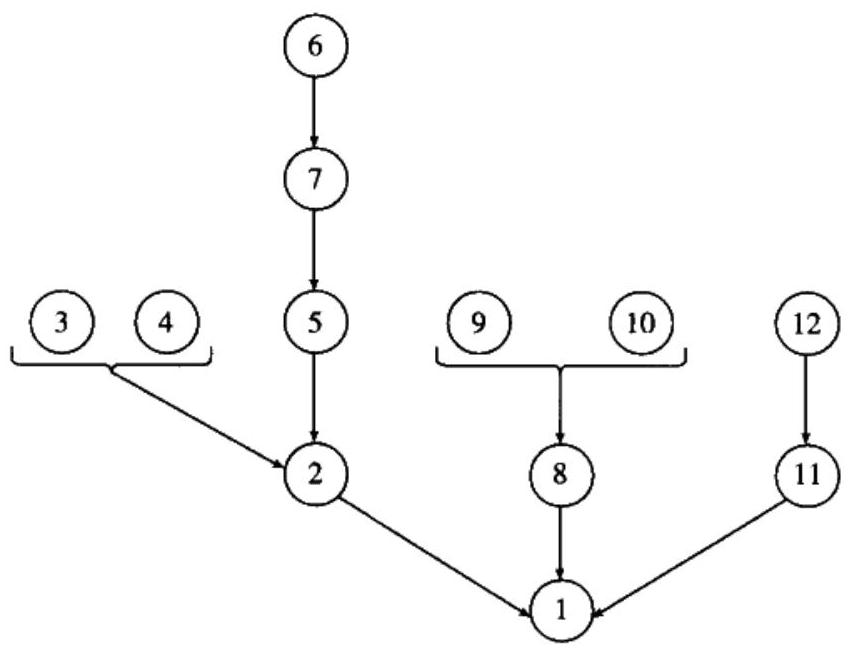
\includegraphics[width=\textwidth]{images/2025_05_15_6a28331d5e7c993ad07ag-076.jpg}
\end{center}

\subsection{逻辑分析的价值}

然而,\logicwarn{日常生活中的论证往往达不到如此高的水准}。它们可能存在以下问题:
\begin{itemize}
  \item 包含作用不明确的陈述
  \item 陈述之间的逻辑连接混乱或错误
  \item 论证者本身思路不清晰
  \item 缺乏系统的推理结构
\end{itemize}

\begin{theorembox}[title=图示法逻辑分析的功能]
\logicemph{诊断功能}:
\begin{itemize}
  \item \logicterm{暴露结构缺陷}:识别推理中的薄弱环节
  \item \logicterm{澄清逻辑关系}:明确前提与结论的真实联系
  \item \logicterm{发现遗漏}:找出论证中缺失的关键环节
\end{itemize}

\logicemph{评估功能}:
\begin{itemize}
  \item \logicterm{判断有效性}:评估推理的逻辑正确性
  \item \logicterm{识别优缺点}:全面分析论证的强弱之处
  \item \logicterm{指导改进}:为论证优化提供方向
\end{itemize}
\end{theorembox}

\logicemph{逻辑学的实践价值}:对实际论证的评估是逻辑学的重要应用领域。成功的评估需要对所分析论证的结构有清楚的把握,而图示法正是实现这一目标的有效工具。

\chaptersummary{
复杂论证性语段在现实中广泛存在,它们具有多层次结构和命题的多重角色特征。\logicterm{图示法}是分析这类语段的重要工具,能够直观展现论证的逻辑结构。

在分析过程中,我们需要处理\logicterm{重复命题}、\logicterm{浓缩前提}等复杂情况,通过系统的分析步骤来理解推理流程。高质量的复杂论证展现出逻辑融贯性,每个命题都有明确作用,共同服务于统一目标。

图示法支持的逻辑分析不仅能够揭示优秀论证的结构特征,更能暴露日常论证中的缺陷,为论证评估和改进提供科学依据。这种分析能力是逻辑学在实际应用中的重要价值体现。
}